
\section{The Standard Model}
The Standard Model (SM)\cite{SMref1,SMref2,SMref3} is the fundamental theory of elementary particle physics. After half a century's development, the Standard Model framework has been confirmed by numerous experiments and can be used to explain most of the data collected about interactions of the fundamental particles. In the Standard Model there are generally 2 categories of particles: fermions and bosons. Fermions, which always have half-integer spins, make up all the matter in the universe. On the other hand, bosons with integer spins mediate the fundamental interactions among the fermions, and the interactions here include the electro-magnetic interaction, the weak interaction and the strong interaction. Figure~\ref{fig:smpfamily} shows all the particles that have been discovered and included in the Standard Model.
\begin{figure}[htbp]
\begin{center}
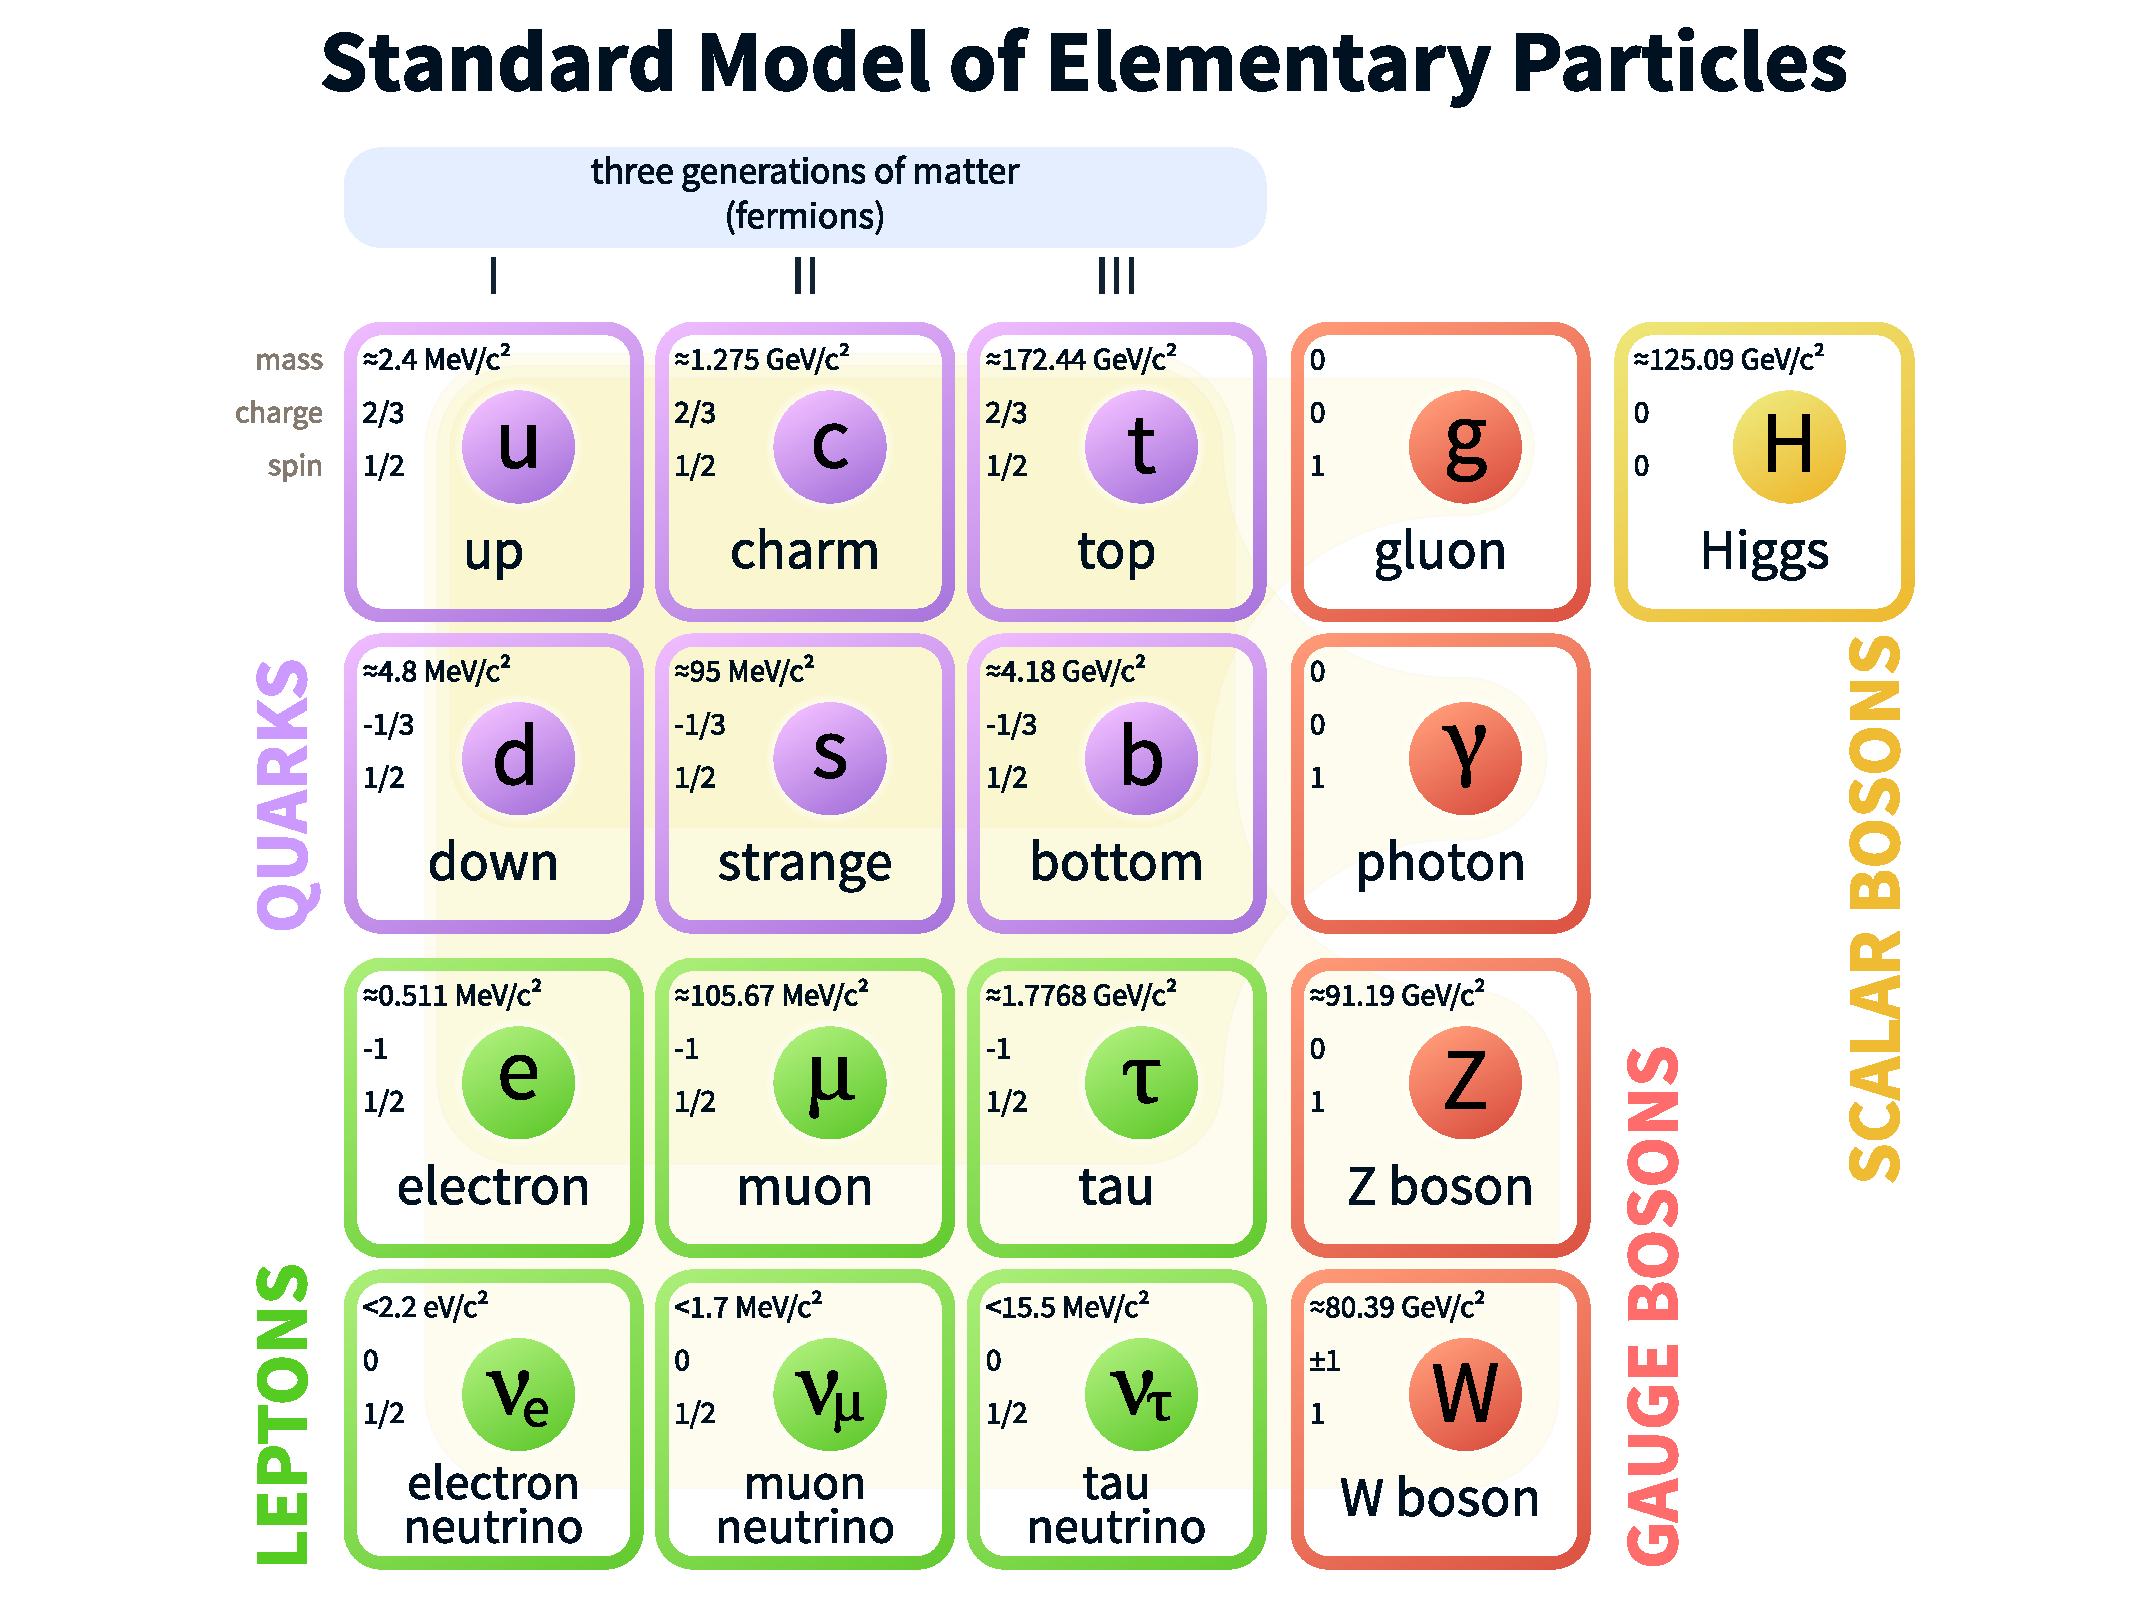
\includegraphics[width=0.72\linewidth]{figures/smpfamily.pdf}
\caption{The Standard Model contains 3 generations of leptons and quarks, 4 kinds of vector bosons and the Higgs boson.}
\label{fig:smpfamily}
\end{center}
\end{figure}

\subsection{Fermions}
Fermions are particles that follow Fermi–Dirac statistics and obey the Pauli exclusion principle. Every fermion has its anti particle, which is a fermion with opposite charge but same mass and spin. The elementary fermions in the Standard Model include leptons and quarks, both of them consist of 3 generations and each generation consists of 2 flavors of fermions. Every elementary fermion in the Standard Model has a spin of one half.
\subsubsection{Lepton}
The leptons do not participate in the strong interaction. There are 3 generations of leptons, and each generation consists of two flavors of leptons: one charged lepton, and one neutral lepton also known as a "neutrino". The charged lepton always carries 1 unit of elementary electric charge, negative for a lepton and positive for its anti-lepton. The masses of the charged leptons have been precisely measured as shown in Figure~\ref{fig:smpfamily}. In the SM, neutrinos are regarded to be massless.

\vspace{0.3cm}
The first generation of leptons includes the electron ($e^{-}$) and electron-neutrino ($\nu _{e}$). Both electron and electron-neutrino have an electron number $L_{e}=1$, while their anti leptons have $L_{e}=-1$. The second generation leptons, the muon ($\mu$) and muon-neutrino ($\nu_{\mu}$), have a muon number $L_{\mu}=1$, while $L_{\mu }=-1$ for the anti-muon ($\bar{\mu}$) and anti-muon-neutrino ($\bar{\nu} _{\mu }$). Similarly, the third generation consists of the tau ($\tau$) and tau-neutrino ($\nu _{\tau }$), with a tau number $L_{\tau}$ accordingly.

\vspace{0.3cm}
In the SM, under the assumption that neutrinos are massless, the lepton numbers are strictly conserved in any kind of interaction. However, recent experiments~\cite{neutrinoOscillation1,neutrinoOscillation2} indicate that the neutrinos have small masses, which implies the lepton numbers can be mixed among different generations.
\subsubsection{Quark}
A quark can participate in any of the 3 interactions in the Standard Model. Like leptons, quarks fall into 3 generations, and each generation contains 2 flavors of quarks having 2/3 and -1/3 elementary electric charge correspondingly. Besides electric charge, quarks also have another intrinsic property known as color charge. The color charge a quark carries is typically defined to be red, blue or green, while the anti quark carries a corresponding anti-color. Quarks are never observed directly in an isolated state due to the phenomenon of color confinement, which confines quarks to only exist in composite, colorless particles known as hadrons.

\vspace{0.3cm}
The first generation includes up and down quarks, the second generation includes charm and strange quarks, and the third generation consists of top and bottom quarks. Every quark has its anti quark, with opposite charge. The mass for each quark is shown in Figure~\ref{fig:smpfamily}. It is possible for heavier quarks to decay into lighter quarks through the weak interaction, especially for quarks within the same generation.
\subsection{Bosons and the interactions}
In contrast to fermions, bosons are particles that follow Bose–Einstein statistics allowing multiple particles in the same state. In the SM there are 4 kinds of vector bosons each with spin 1 and one spin-0 scalar boson, which is the recently discovered Higgs boson. The vector bosons work as force carriers of the 3 interactions, while the masses of the elementary particles are generated by their interaction with the Higgs field.
\subsubsection{Vector Bosons}
In the SM, the vector bosons (gluon, photon, Z boson and W boson) work as mediators of the 3 fundamental interactions among fermions. Each of the vector bosons has spin 1.
\begin{itemize}
\item the \textbf{gluon} is the force mediator of the strong interaction, described in Quantum Chromodynamics (QCD) theory, a gauge theory based on SU(3). Gluons are massless and have no electric charge.
\item the \textbf{photon} is the force mediator of the electromagnetic interaction, described in Quantum Electrodynamics (QED) theory, a $U(1)_{EM}$ theory. Photons are massless and have no electric charge.
\item the \textbf{Z boson} is the mediator of the weak interaction with no electric charge flow. The Z boson has no charge, while it has mass of 91.2\GeV, which makes it possible to decay into a fermion–antifermion pair.
\item the \textbf{W boson} is the mediator of the weak interaction with electric charge flow. The W carries either 1 or -1 elementary electric charge, denoted as $W^{+}$ and $W^{-}$, both having masses of 80.4\GeV. Like the Z boson, W bosons can decay into fermion–antifermion pairs.
\end{itemize}
In the SM, the unification of the electromagnetic and weak interactions is realized by an SU(2) $\times$ U(1) gauge group. The photon, Z boson and W boson are generated in the SU(2) $\times$ U(1) group due to the process of spontaneous symmetry breaking described by the Higgs mechanism. 
\subsubsection{The Higgs Boson}
In the 1960s the Higgs boson and Higgs mechanism was proposed in order to explain the source of the masses of the gauge bosons\cite{higgstheory1,higgstheory2,higgstheory3}, which are expected to be massless according to the gauge theory. That assumption clearly conflicts with the experiment facts. The Higgs mechanism suggests that an SU(2) doublet of complex scalar fields breaks the SU(2) symmetry as its potential in the form of $\mu^{2}\phi^{\dagger}\phi + \lambda^{2}(\phi^{\dagger}\phi)^2$ with $\mu^{2}<0$ and $\lambda^{2}>0$ leads to a non-zero vacuum expectation value which does not follow the SU(2) symmetry. This phenomenon is referred to as "spontaneous symmetry breaking" and the field here is the Higgs field. Due to the spontaneous symmetry breaking, three gauge bosons gain masses when interacting with the scalar field, and the Higgs Boson comes from one degree of freedom of the field while the other 3 degrees are no longer observable.

\vspace{0.3cm}
On July 4 of 2012, the discovery of the Higgs boson was announced by both the CMS and ATLAS Collaborations at the CERN, LHC\cite{higgsdiscover1,higgsdiscover2}. Hence the Higgs boson officially became one member of the standard model elementary particle family. The Higgs boson has no spin or electric charge, and its mass is measured to be 125\GeV. It is very unstable and mainly decays into a $b\bar{b}$ quark pair, $\tau\bar{\tau}$ pair or off shell gauge boson pair.

\section{The Limitations of SM and the Hierarchy Problem}
Although the SM has been tested and demonstrated as a great success among numerous particle physics experiments and provides reliable physics predictions for most of the sceneries, it is not yet believed to be a complete theory. The SM does not provide theoretical support for either dark energy or dark matter particles which are believed to exist according to cosmological observations. Moreover, within the SM particles, neutrino oscillation proved by several experiments conflicts with the SM's assumption of massless neutrinos. Above all, as mentioned above, the SM incorporates only 3 of the 4 fundamental interactions, leaving gravitation completely unexplained in the scope of particle physics.

\vspace{0.3cm}
The Hierarchy Problem~\cite{intro_hierarchy} in particle physics refers to the huge discrepancy between the electroweak scale and the gravitational scale, as the weak force is about $10^{24}$ times stronger than gravity. The Fermi's constant denoting the scale of the weak interaction is expected to be smaller and closer to the Newton's constant for gravity, based on the calculation of SM. In other words, we expect the large quantum contributions to the square of the Higgs boson mass would make the Higgs boson much heavier than the measured 125\GeV. It could be that the measured Higgs boson mass is the result of incredibly fine-tuned constants within the SM. Alternatively, some new theoretical mechanism is expected. The Bulk RS Graviton Model is one of the possible solutions.

\section{Bulk RS Graviton Model}
The Bulk RS Graviton model offers an efficient solution to the Hierarchy problem. It also provides theoretical support for the production of heavy di-boson resonances, which can result from interactions involving an extra spatial dimension. The development and features of this model are summarized below.
\subsection{Introduction of Extra Dimension Models}
In the 1920s, the Kaluza–Klein theory was proposed as a means to unify gravitation and electromagnetism. It assumed a 5th dimension beyond our usual four dimension of space and time and started purely from the 5 dimensional extension of General Relativity. The quantum mechanical interpretation predicts that gravitons or other particles in the extra dimension will acquire quantized excited modes, which are referred to as Kaluza-Klein (K-K) modes. The K-K theory is considered an important precursor to subsequent theories that introduce extra spatial dimensions as a solution to the Hierarchy Problem.

\vspace{0.3cm}
Following the K-K theory, a number of extra dimension theories were proposed attempting to address the Hierarchy problem, such as the ADD model. The ADD model~\cite{Intro_ADD,Intro_ADD2} was proposed in 1998 by Nima Arkani-Hamed, Savas Dimopoulos, and Gia Dvali, suggesting the existence of additional large extra spatial dimensions. It proposed that the Planck scale $M_{Pl}(\sim{G_{N}}^{-1/2})$ is not a fundamental scale but is instead simply a consequence of the large size of the new dimensions. While gravitons can freely propagate in the new dimensions, at sub-weak energies the SM fields must be localized to a 4-dimensional manifold of weak scale thickness in the extra dimensions. 

\subsection{Randall–Sundrum Model}
The Randall-Sundrum (RS) model~\cite{Intro_RS1} was originally proposed in 1999 by Lisa Randall and Raman Sundrum, because they were not satisfied with those large extra dimension models that involved fine tunings of the bulk cosmological constant and brane tensions. This theory is often referred to as the RS1 model. The framework is based on a slice of 5-dimensional anti-de Sitter space ($AdS_{5}$)~\cite{Intro_ads5}, with two flat four-dimension branes on each boundary. According to the $AdS_{5}$ theory, if the flat 4D branes carry energy, the geometry of the additional dimension has to be warped to be consistent with the General Relativity. The line segment ($ds$) which determines the distance scale is given by equation~\ref{eqn:intro_ds},
\begin{equation}
ds^2 = e^{-2ky}{\eta}_{\mu\nu}{dx}^{\mu}{dx}^{\nu}+dy^2,
\label{eqn:intro_ds}
\end{equation}
where ${\eta}_{\mu\nu}$ is the Minkowski metric for flat four-dimension space; ${dx}^{\mu}$ is the regular time-space four-vector; $y$ represents the 5th dimension coordinate, bounded by $0\leq y \leq \pi R$ and $R$ is the extra dimension length; $k$ is the curvature constant.

\vspace{0.3cm}
Fluctuations on 2 of the variables are possible, $k$ and $R$, each corresponding to a particle field: the graviton and radion. In the RS1 model, the SM particles are all trapped on one of the branes, referred to as the TeV Brane, located at $y=\pi R$. The other brane in this model, named the Plank Brane and located at $y=0$, has a Planckian fundamental scale and is the brane where the 4D (or zero-mode) graviton concentrates. Given this assumption, it is possible to unify the fundamental gravitational and weak mass scales, since the 4D physical masses on the TeV brane acquire an exponential rescaling of $e^{-2ky}$. Figure~\ref{fig:intro_branes} gives the idea of this extra dimension model and the metric behavior.
\begin{figure}[htbp]
\begin{center}
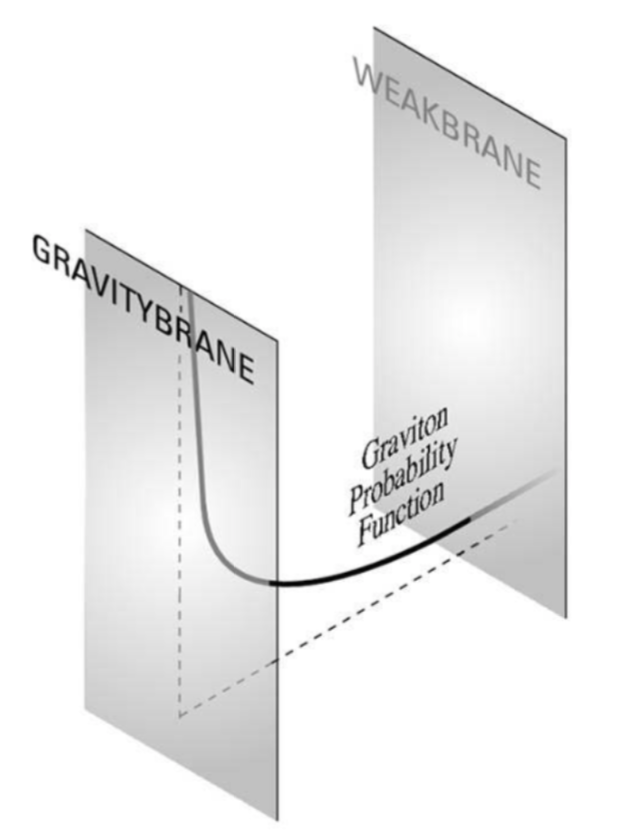
\includegraphics[width=0.32\linewidth]{figures/intro_branes.png}
\caption{In RS theory, the Gravity Brane (Planck Brane) and the Weak Brane (TeV Brane) are the 4 dimensional boundaries of the extra dimension. The metric behavior along the extra dimension is also shown.}
\label{fig:intro_branes}
\end{center}
\end{figure}

The key feature of the RS1 model is that, though the zero-mode spin-2 graviton is localized in the Plank Brane, its K-K excited mode (K-K graviton) is localized near the TeV brane and has mass around a TeV, so that K-K graviton coupling to the entire SM is only $\sim$ TeV suppressed.
\subsection{The Bulk RS Graviton Model}
However, in the RS1 model, the higher-dimensional operators in the 5D effective field theory are suppressed only by the warped scale $\sim$ TeV, giving contributions that are too large to flavor-changing neutral current (FCNC) processes~\cite{intro_rsfcnc1,intro_rsfcnc2} which are strongly suppressed in the SM.

\vspace{0.3cm}
A solution to this issue is to allow the SM fields to propagate in the extra dimension, which leads to the scenario of the Bulk RS Graviton model~\cite{intro_bulkref1,intro_bulkref2,intro_bulkref3}. In this model, the SM particles are identified with the zero-modes of the 5D fields and the profile of a SM fermion in the extra dimension depends on its 5D mass parameter. We can then choose to localize 1st and 2nd generation fermions near the Planck brane, so that their interactions to the K-K gauge bosons are suppressed, as the K-K gauge bosons are near the TeV brane and have little overlapping with the light fermions. Therefore,  the FCNCs from higher-dimensional operators are suppressed by scales far beyond TeV scale.

\vspace{0.3cm}
Like the RS1 model, the K-K gravitons are localized near the TeV brane. Figure~\ref{fig:intro_rsandbulk} shows the zero-modes of the SM matter fields and the K-K graviton along the 5th dimension, for the Bulk RS model and RS1 model.
\begin{figure}[htbp]
\begin{center}
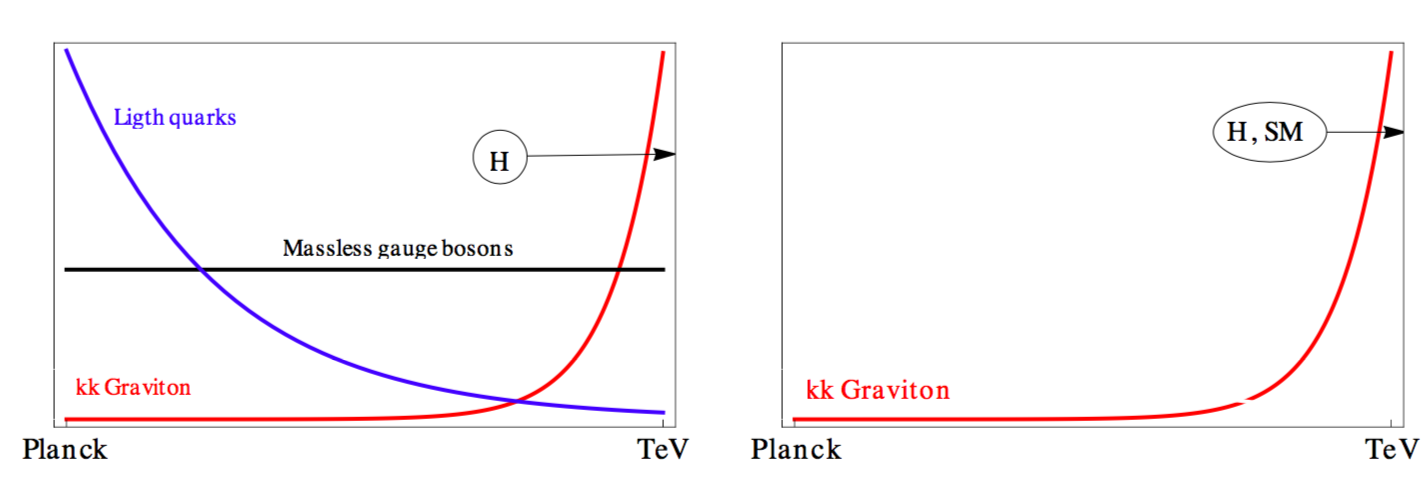
\includegraphics[width=0.9\linewidth]{figures/intro_rsandbulk.png}
\caption{Zero-modes of the SM matter fields and the K-K graviton along the extra dimension for the Bulk RS model scenario (left), and RS1 (right).}
\label{fig:intro_rsandbulk}
\end{center}
\end{figure}

From Figure~\ref{fig:intro_rsandbulk} one can see that in the Bulk RS scenario the light fermions are localized near the Plank brane while the K-K gravitons are near the TeV brane, as a result, the couplings of the K-K gravitons to light fermions are highly suppressed compared to the RS1 model. Additionally, the SM massless gauge bosons have flat distribution across the extra dimension, which also leads to the suppression of their couplings to the K-K gravitons by roughly a factor of $k\pi R$.

\subsection{Phenomenology of the Bulk Graviton Model}
As in the RS1 model, there are 2 free parameters in the RS Bulk theory, the curvature constant $k$ and the extra dimension length $R$. Equivalently they can be expressed as $\tilde{k}$, which is defined as the ratio of $k$ and the reduced Plank mass ($\overline{M_{Pl}}\equiv M_{Pl}/\sqrt{8\pi}$), and the K-K graviton mass ($m_{G}$). The K-K Graviton in the Bulk Graviton model can be produced in several ways, while the dominant process is QCD gluon fusion. Figure~\ref{fig:intro_Gxsec} shows the cross sections for the production of a Bulk Graviton production for different processes, with $\tilde{k}=0.1$ and proton-proton center of mass energy of 13TeV.
\begin{figure}[htbp]
\begin{center}
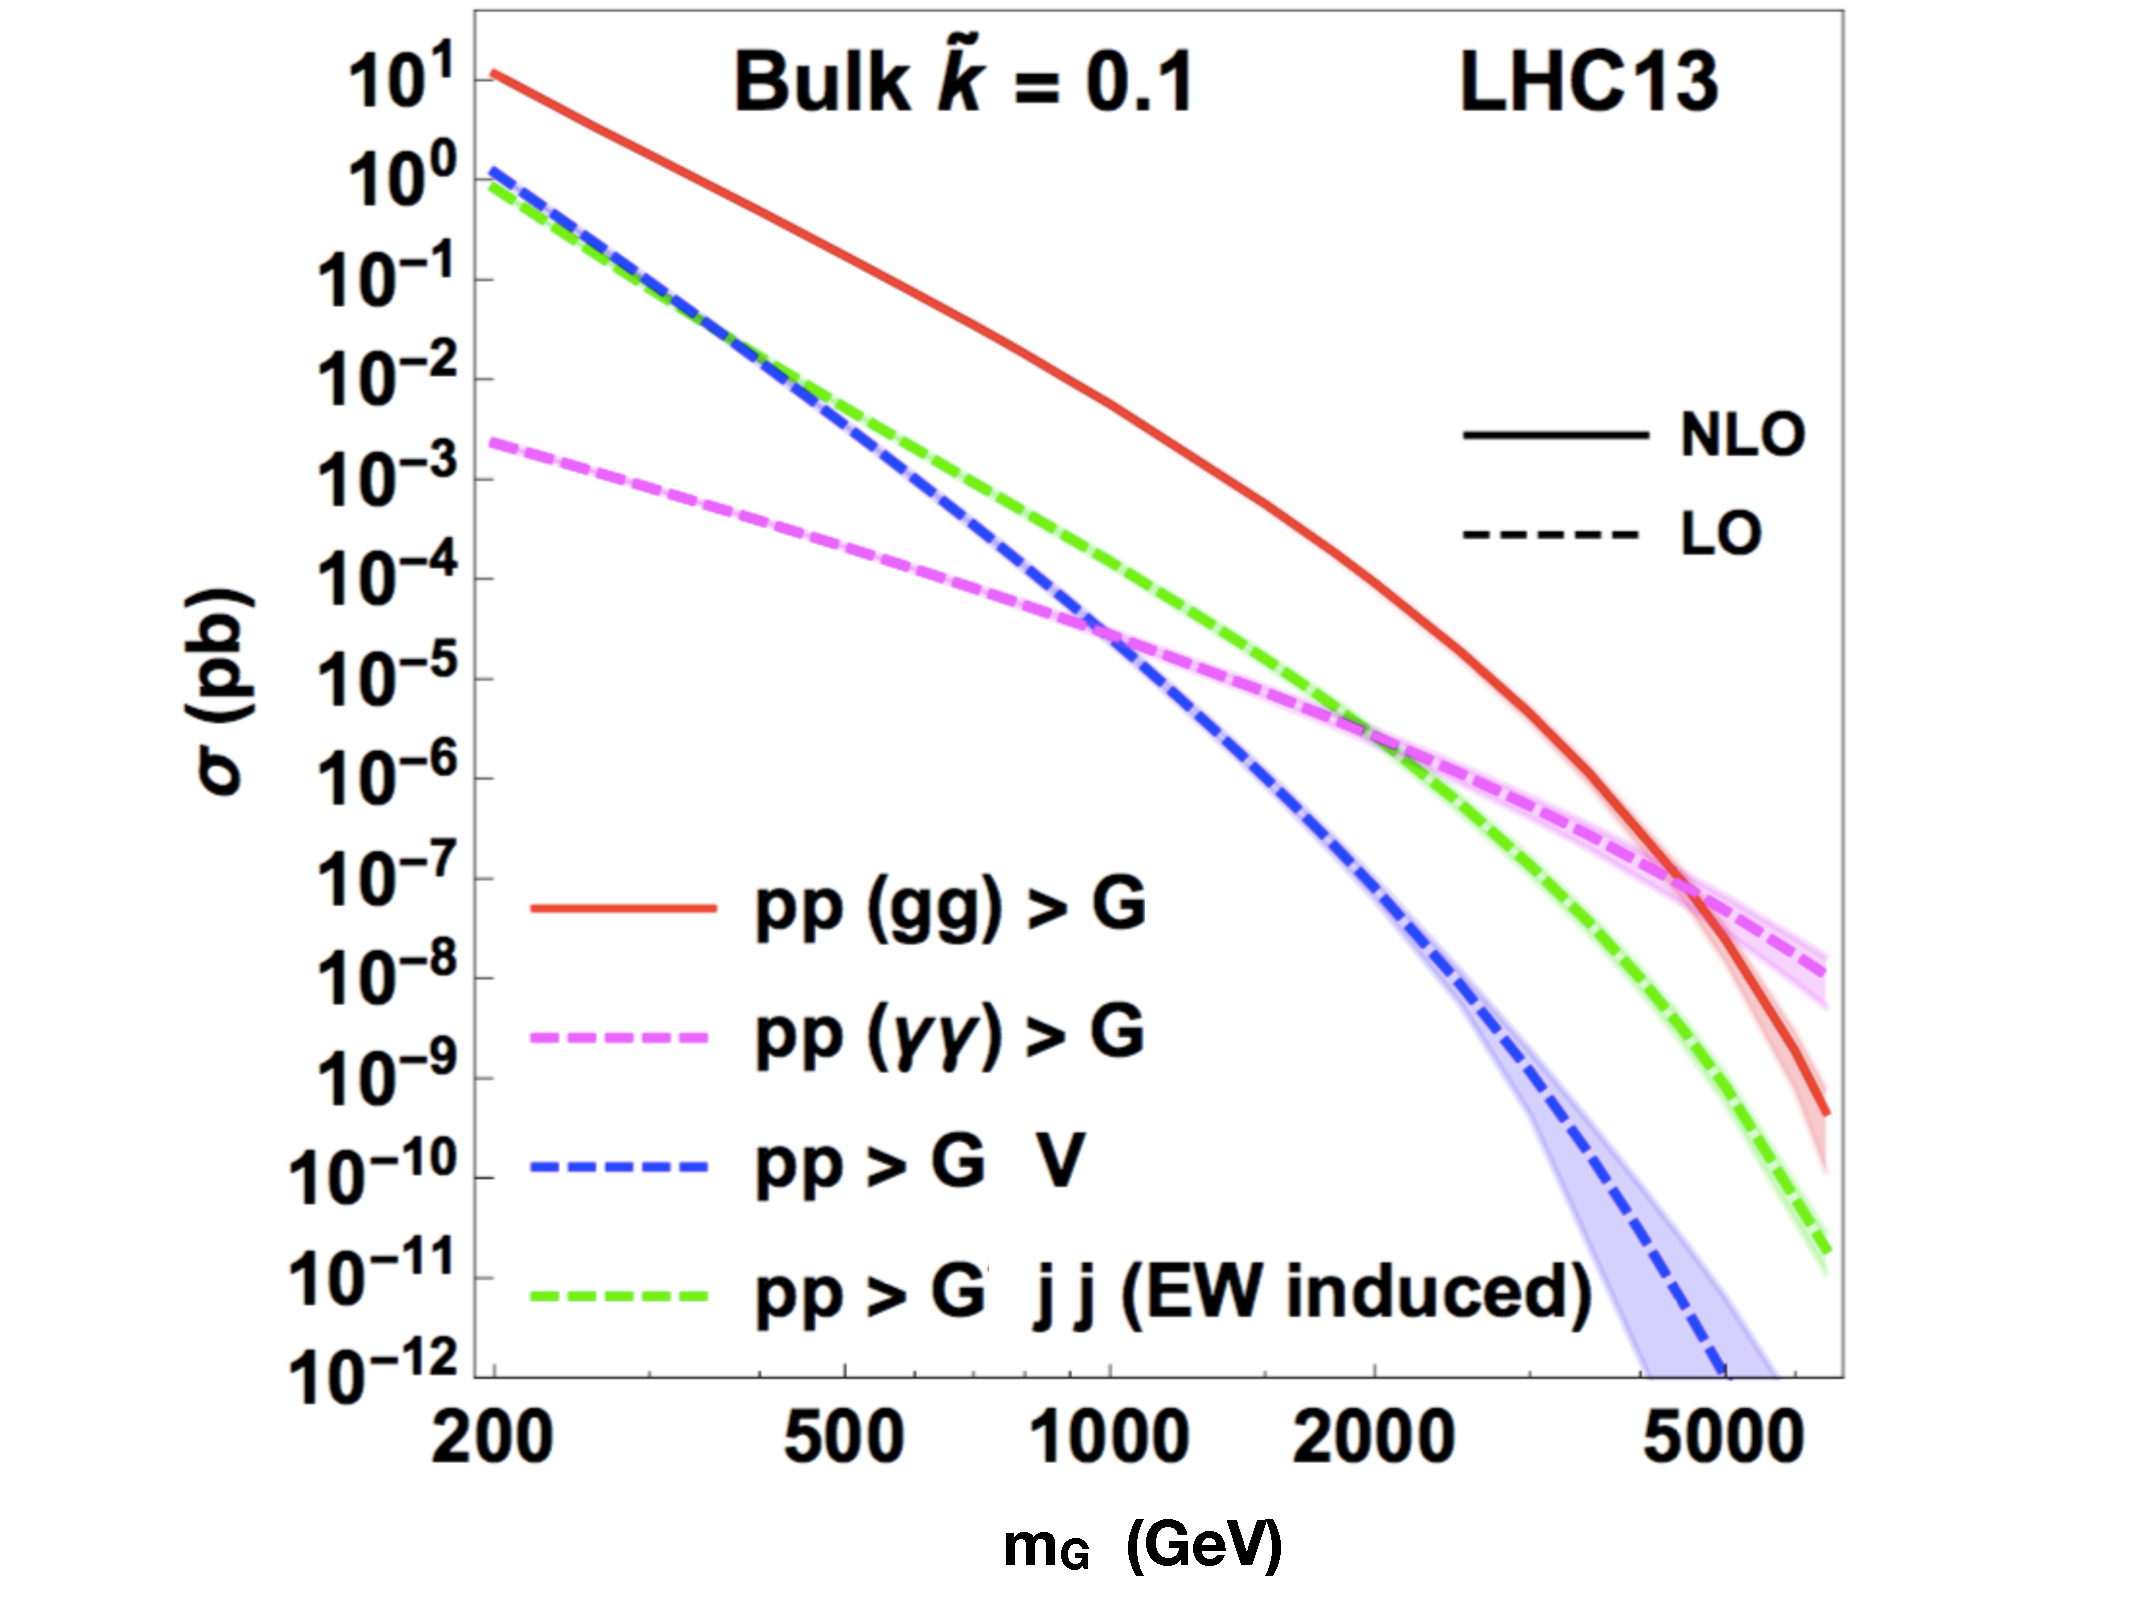
\includegraphics[width=0.5\linewidth]{figures/intro_Gxsec.pdf}
\caption{Production cross section for the K-K Graviton in the Bulk RS model, $\tilde{k}=0.1$}
\label{fig:intro_Gxsec}
\end{center}
\end{figure}
Here the $pp\rightarrow Gjj$ mode is dominated by the Vector Boson Fusion (VBF) process, and the $pp\rightarrow GV$ denotes the associated production with a massive vector boson. For $\tilde{k}<1$ and $m_{G}<2$ TeV the width of the K-K graviton is less than 6\% of the graviton mass, therefore a narrow resonance is expected. In this case the production cross section scales with $\tilde{k}$ as described in Equation~\ref{eqn:intro_kxsec}.
\begin{equation}
\sigma (m_G,\tilde{k}) = (\tilde{k}/0.1)^2 \sigma (m_G,\tilde{k}=0.1)
\label{eqn:intro_kxsec}
\end{equation}

In terms of the decay modes, the K-K gravitons are most likely to decay to SM particles localized near the TeV brane, as they have the strongest coupling to the graviton. Therefore the dominant decay modes are to top quarks and Higgs, as well as Z and W bosons, while the decay modes into massless gauge bosons and light quarks are suppressed and negligible. Figure~\ref{fig:intro_Gbr} shows the branching ratios for the decay of a Bulk Graviton.
\begin{figure}[htbp]
\begin{center}
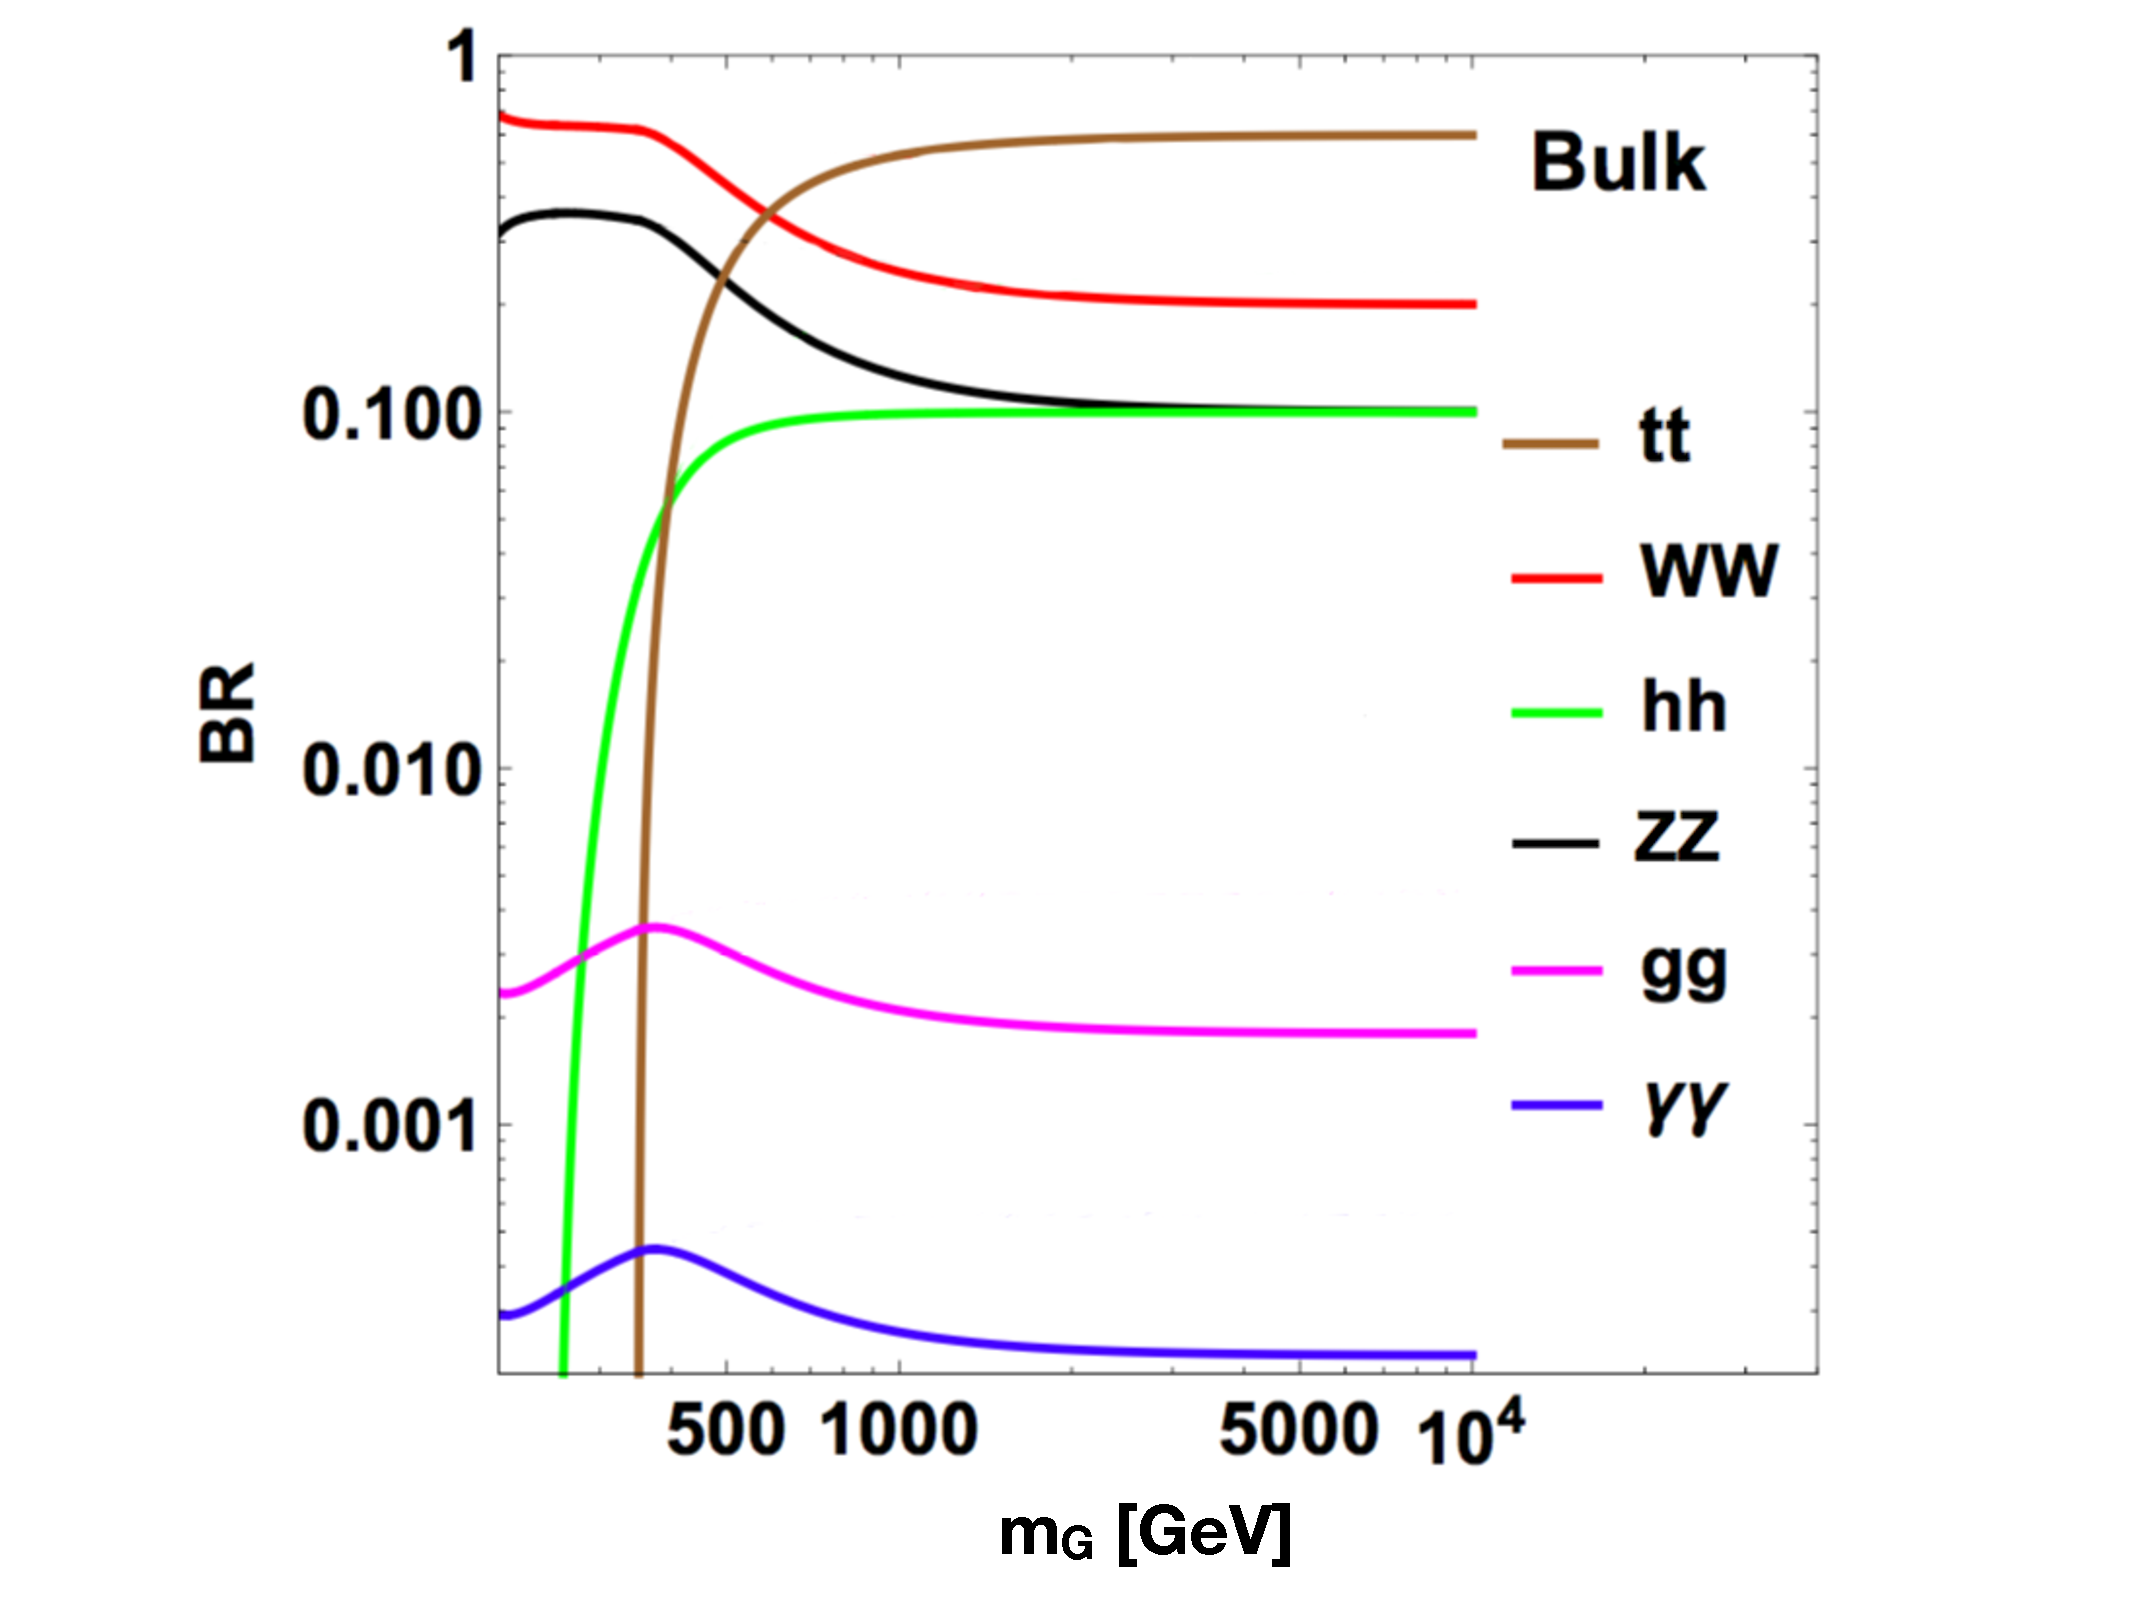
\includegraphics[width=0.5\linewidth]{figures/intro_Gbr.pdf}
\caption{Branch fraction of Bulk Graviton decay modes.}
\label{fig:intro_Gbr}
\end{center}
\end{figure}
The decay branching fractions are independent of $\tilde{k}$. Although the top channel and h channel have the highest branch fractions, neither of these channels can be easily detected or reconstructed. In contrast, despite of the relatively lower branching ratio, the W and Z boson channels are more preferred for the experimental search.

\section{Status of Searches for the Bulk Graviton} 
As described above, the Bulk Graviton can be produced by gluon fusion as well as other processes occurring in proton-proton collisions produced at the Large Hadron Collider. Because of the large gluon luminosity at the LHC, these data are ideally suited to search of evidence of a Bulk Graviton.
\subsection{Previous Searches}
Previous searches~\cite{Aad:2012nev,Aad:2013wxa,Aad:2014xka,Chatrchyan:2012baa,Khachatryan:2014gha,Aaboud:2016okv} for the Bulk Graviton have been performed based on data collected from both ATLAS and CMS detectors with the proton-proton center of mass energy at 7, 8 and 13\GeV. Limits on the cross section for the production of a Bulk Graviton have been set as a function of $m_{G}$. The existence of the Bulk Graviton was excluded with mass below 610\GeV~\cite{Chatrchyan:2012baa} for $\tilde{k}=0.5$ and mass below 1100\GeV~\cite{Aaboud:2016okv} for $\tilde{k}=1.0$ at 95\% confidence level. In these searches, semi-leptonic final states including leptons and jets, comprise the most popular channels. There is no previous search studying the channel ZZ to $2\ell 2\nu$.
\subsection{\boldmath{$2\ell 2\nu$} channel and  Search Strategy}
In this analysis we present a search for the Bulk Graviton or similar resonances decaying into a pair of Z bosons, in which one of the Z boson decays into a pair of charged leptons, either an electron pair or a muon pair (denoted by "$\ell$"), while the other decays into two neutrinos (denoted by "$\nu$"). Figure~\ref{fig:intro_llnndiagram} shows the Feynman diagram of this process. This analysis is based on the data from proton-proton collisions at a center-of-mass energy of 13 TeV collected by the CMS detector in 2016 and corresponding to an integrated luminosity of 35.9 fb$^{-1}$. 
\begin{figure}[htbp]
\begin{center}
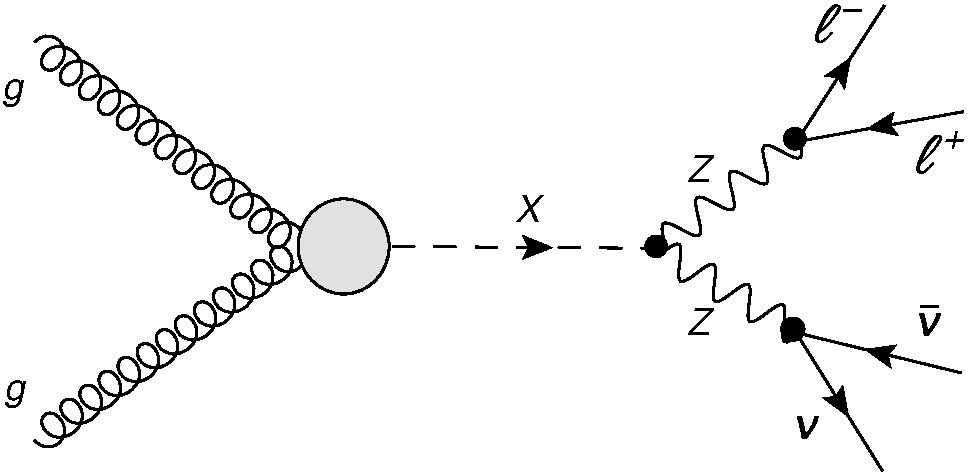
\includegraphics[width=0.72\linewidth]{figures/intro_llnndiagram.pdf}
\caption{Leading order Feynman diagram for the production of resonance X via gluon–gluon fusion decaying to the ZZ$\rightarrow 2\ell 2\nu$ final state}
\label{fig:intro_llnndiagram}
\end{center}
\end{figure}
The signature of the  $2\ell 2\nu$ channel is a pair of adjacent leptons with high transverse momentum ($p_T$) from the decay of a boosted Z boson and large missing transverse momentum from the other Z boson decaying to neutrinos, which is denoted as \ptmiss.

\vspace{0.3cm}
Compared to the semi-leptonic channels, the $2\ell 2\nu$ channel has reduced background. Although \Zjets production is a main source of background for both of these channels, it is almost impossible to distinguish the ZZ to $2\ell 2q$ process from \Zjets background, as they have very similar kinematics -- a Z boson and corresponding hadronic recoil. Unlike the \Zjets background, events from the ZZ to $2\ell 2\nu$ process always includes large \ptmiss, which makes it possible to strongly suppress the \Zjets background. Although the $2\ell 2q$ channel has a larger branching fraction, the branching fraction of the $2\ell 2\nu$ is still considerable, about 1/3 of that of the $2\ell 2q$ channel and 6 times as large as that for the four charged-lepton final state. The combination of lower statistics and the effects on resolution of a signal due to the undetected neutrinos explains why no previous search in $2\ell 2\nu$ channel was carried out. But now in RunII data with larger cross section from the higher collision energy and the larger and growing statistics, the $2\ell 2\nu$ channel has become more advantageous.

\vspace{0.3cm}
Because of the invisible neutrinos from the second Z boson decay, we will not have full momentum information for that Z boson, instead, only \ptmiss is available, which can be observed as the projection of the invisible Z boson's momentum on the x-y detector plane. Therefore it is not possible to reconstruct the invariant mass of the $2\ell 2\nu$ system. In this analysis the transverse mass ($m_{T}$) is designated as the discriminating variable to separate signal from background. The transverse mass variable is defined as:
\begin{equation}
m_{T}^2 = \left[ \sqrt{({p_{T}}^{\ell\ell})^2 + m^2_{\ell\ell}}
      + \sqrt{({p_{T}}^{miss})^2+m^2_{\ell\ell}}\right]^2
      - \left[\vec{p}_{T}^{\ell\ell}+\vec{p_{T}}^{miss}\right]^2,
\label{eqn:intro_MT}
\end{equation}

Here ${p_{T}}^{\ell\ell}$ and $m_{\ell\ell}$ each represent the $p_{T}$ and mass of the Z boson constructed from the charged lepton pair system. The $m_{\ell\ell}$ in the middle term provides an estimator of the mass of the invisibly decaying Z boson. This choice has negligible impact on the expected signal at large $m_{T}$, but is found to preferentially suppress backgrounds from $t\bar{t}$ and WW decays.

\vspace{0.3cm}
Although the $m_{T}$ variable only equals the invariant mass confined to the transverse plane, a kinematic edge is still expected from the putative heavy resonance, and the position of the edge strongly depends on the mass of the resonance. Figure~\ref{fig:intro_mt} gives an example of what the transverse mass spectrums look like from the decay of resonances with invariant masses each at 800\GeV, 1000\GeV, 1200\GeV and 1400\GeV. The kinematic edges on the right side of each spectrum are very close to the graviton mass values.

\begin{figure}[htbp]
\begin{center}
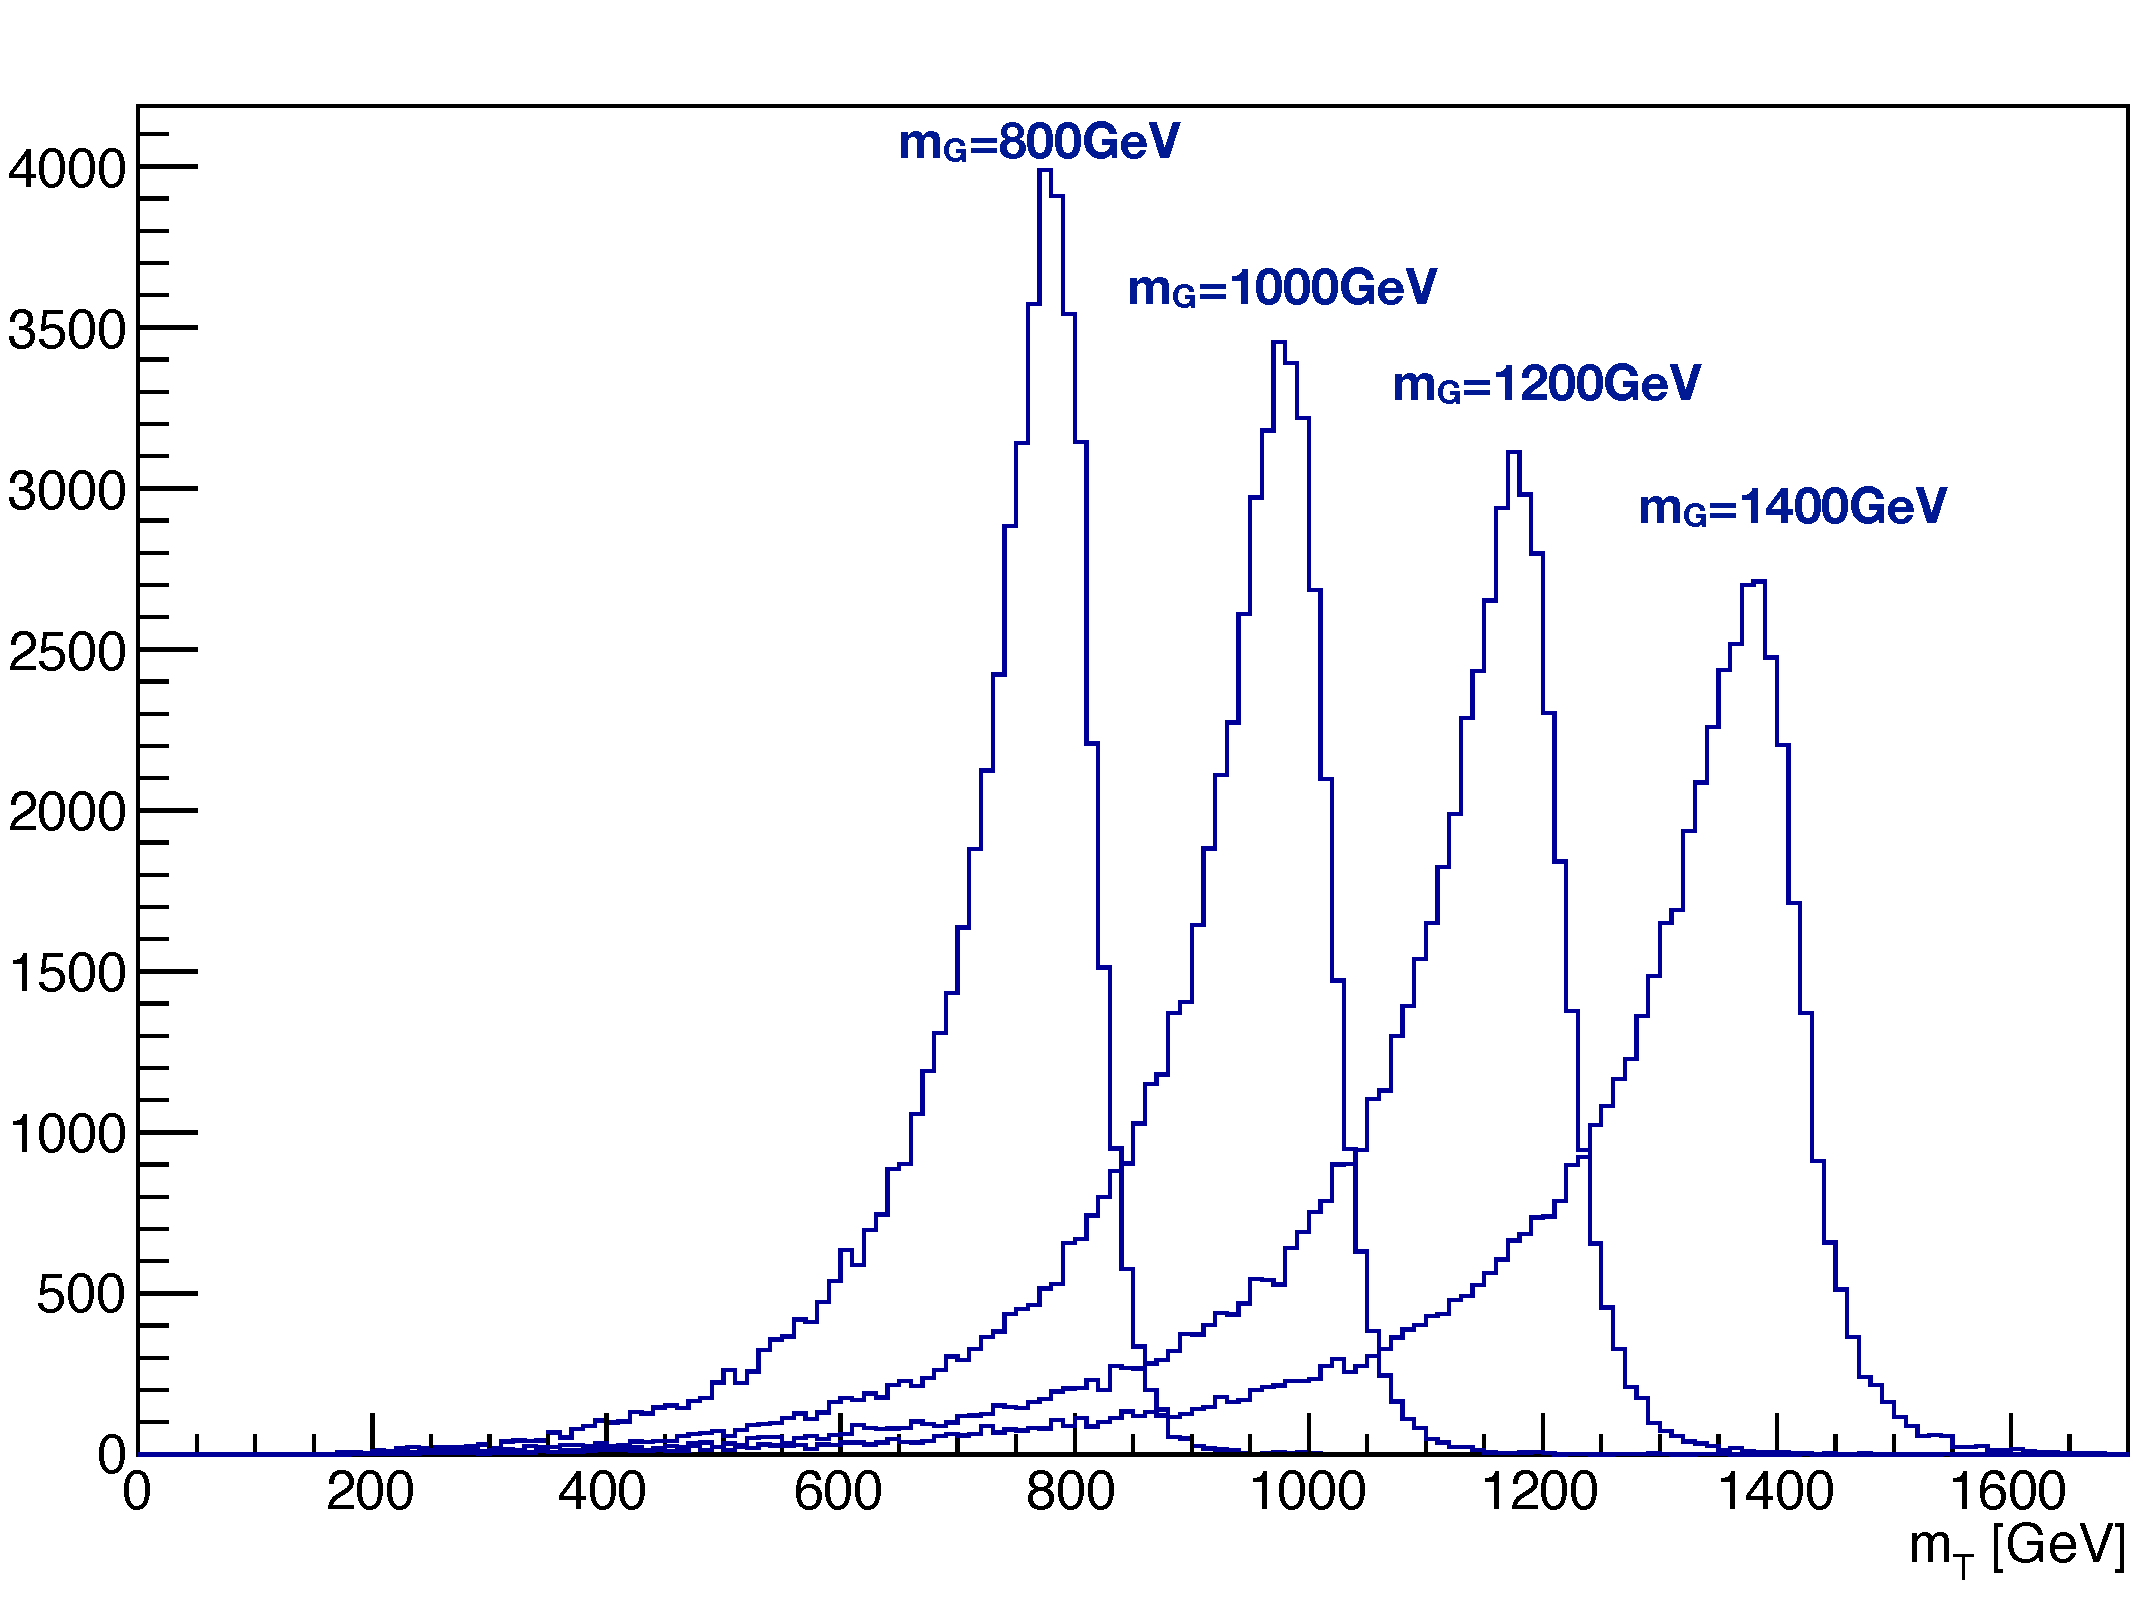
\includegraphics[width=0.72\linewidth]{figures/intro_example_mt.pdf}
\caption{The transverse mass($m_{T}$) spectrums of resonances with masses at 800\GeV, 1000\GeV, 1200\GeV and 1400\GeV.}
\label{fig:intro_mt}
\end{center}
\end{figure}

\vspace{0.3cm}
The transverse mass can also be written in an alternate form in which no vector is involved:
\begin{small}
\begin{equation}
m_{T}^2 = \left[ \sqrt{({p_{T}}^{\ell\ell})^2 + m^2_{\ell\ell}}
      + \sqrt{({p_{T}}^{miss}_\perp)^2+({p_{T}}^{miss}_\parallel)^2+m^2_{\ell\ell}}\right]^2
      - \left({p}_{T}^{\ell\ell}+{p_{T}}^{miss}_\parallel\right)^2
      - ({p_{T}}^{miss}_\perp)^2,
\label{eqn:intro_MTalt}
\end{equation}
\end{small}
where ${p_{T}}^{miss}_\parallel$ refers to the projection of \ptmiss in the direction of ${p}_{T}^{\ell\ell}$ and ${p_{T}}^{miss}_\perp$ is the fraction perpendicular to ${p}_{T}^{\ell\ell}$.

%\section{CMS and Me} %what did i do in this analysis and others
%In August 2014, I joined the UVA CMS group and worked on calibrating a prototype Shashlik calorimeter using the muon data as my first project here. Aferwards, in the middle of 2015, I left for CERN, Switzerland and stayed there for 2 years. During my stay at CERN I was involved in several projects and activities both on the detector and physics analysis. 

%\vspace{0.3cm}
%My most detector-related work focused on the Hadron Calorimeter(HCAL). Starting with the Hadron Forward (HF) detector frontend electronics Phase I upgrade in 2015. I joined the HCAL upgrade team, helping design and carry out a series of electronics tests. In 2016 I helped the HCAL Endcap (HE) upgrade with the system monitoring, and HCAL Data Quality Management (DQM) group with their online DQM system for the HF/HE upgrades. I was also taking the HCAL detector on call expert shifts continually for 1 year and a half since 2016.

%\vspace{0.3cm}
%In terms of physics analysis, I started working on this di-boson analysis in the December of 2015, helping to design and implement the analysis framework from scratch, studying the pileup reweighting, trigger efficiency, lepton identification algorithms and their efficiencies, as well as determining the non-resonant background using data-driven modeling. The muon tracker High $p_{T}$ efficiency calculated by me has been widely used in related CMS analyses and I am also contributing to the high $p_{T}$ muon paper carried out by the muon Physics Object Group (POG). Apart from this di-boson analysis, I also worked as the generator contact person for physics simulations in the Beyond Two Generations (B2G) Physics Analysis Group (PAG) for the whole year of 2017.
